\documentclass[12pt]{article}
\usepackage[top=1in,left=1in, right = 1in, footskip=1in]{geometry}

\usepackage{graphicx}
\usepackage{xspace}
%\usepackage{adjustbox}

\newcommand{\comment}{\showcomment}
%% \newcommand{\comment}{\nocomment}

\newcommand{\showcomment}[3]{\textcolor{#1}{\textbf{[#2: }\textsl{#3}\textbf{]}}}
\newcommand{\nocomment}[3]{}

\newcommand{\jd}[1]{\comment{cyan}{JD}{#1}}
\newcommand{\swp}[1]{\comment{magenta}{SWP}{#1}}
\newcommand{\bmb}[1]{\comment{blue}{BMB}{#1}}
\newcommand{\djde}[1]{\comment{red}{DJDE}{#1}}

\newcommand{\eref}[1]{Eq.~\ref{eq:#1}}
\newcommand{\fref}[1]{Fig.~\ref{fig:#1}}
\newcommand{\Fref}[1]{Fig.~\ref{fig:#1}}
\newcommand{\sref}[1]{Sec.~\ref{#1}}
\newcommand{\frange}[2]{Fig.~\ref{fig:#1}--\ref{fig:#2}}
\newcommand{\tref}[1]{Table~\ref{tab:#1}}
\newcommand{\tlab}[1]{\label{tab:#1}}
\newcommand{\pday}{\ensuremath{/\textrm{day}}}

\usepackage{amsthm}
\usepackage{amsmath}
\usepackage{amssymb}
\usepackage{amsfonts}

\usepackage{lineno}
\linenumbers

\usepackage[pdfencoding=auto, psdextra]{hyperref}

\usepackage{natbib}
\bibliographystyle{chicago}
\date{\today}

\usepackage{xspace}
\newcommand*{\ie}{i.e.\@\xspace}

\usepackage{color}

\newcommand{\Rx}[1]{\ensuremath{{\mathcal R}_{#1}}\xspace} 
\newcommand{\Ro}{\Rx{0}}
\newcommand{\Rc}{\Rx{\mathrm{c}}}
\newcommand{\Ri}{\Rx{\mathrm{i}}}
\newcommand{\RR}{\ensuremath{{\mathcal R}}\xspace}
\newcommand{\Rhat}{\ensuremath{{\hat\RR}}}
\newcommand{\Rprop}{\Rx{\mathrm{prop}}}
\newcommand{\Rcori}{\Rx{\mathrm{cori}}}
\newcommand{\tsub}[2]{#1_{{\textrm{\tiny #2}}}}
\newcommand{\dd}[1]{\ensuremath{\, \mathrm{d}#1}}
\newcommand{\dtau}{\dd{\tau}}
\newcommand{\dx}{\dd{x}}
\newcommand{\dsigma}{\dd{\sigma}}

\newcommand{\tstart}{\ensuremath{\tsub{t}{start}}\xspace}
\newcommand{\tend}{\ensuremath{\tsub{t}{end}}\xspace}

\newcommand{\betaeff}{\ensuremath{\tsub{\beta}{eff}}\xspace}
\newcommand{\Keff}{\ensuremath{\tsub{K}{eff}}\xspace}
\newcommand{\Kpost}{\ensuremath{\tsub{K}{post}}\xspace}

\newcommand{\pt}{p} %% primary time
\newcommand{\st}{s} %% secondary time

\newcommand{\psize}{{\mathcal P}} %% primary cohort size
\newcommand{\ssize}{{\mathcal S}} %% secondary cohort size

\newcommand{\gtime}{\sigma} %% generation interval
\newcommand{\gdist}{g} %% generation-interval distribution

\newcommand{\geff}{g_{\textrm{eff}}} %% generation-interval distribution

\newcommand{\total}{{\mathcal T}} %% total number of serial intervals

\newcommand{\PP}{\ensuremath{\mathcal P}}
\newcommand{\II}{\ensuremath{\mathcal I}}
\newcommand{\HH}{\ensuremath{\mathcal H}}

\begin{document}

\begin{flushleft}{
	\Large
	\textbf\newline{
		Immune boosting bridges leaky vaccine and polarized vaccine models
	}
}
\newline
\\
Sang Woo Park\textsuperscript{1,*}, Chadi Saad-Roy, Irena Papst, ???, Jessica Metcalf, Bryan T Grenfell, Jonathan Dushoff
\\
\bigskip
\textbf{1} Department of Ecology and Evolutionary Biology, Princeton University, Princeton, NJ, USA
\\
\bigskip

*Corresponding author: swp2@princeton.edu
\end{flushleft}

In this study, we compare different models of vaccination.
First, we illustrate that the difference between the leaky vaccination model and the polarized vaccination models can be reconciled via immune boosting mechanism.



\section{Mathematical models of vaccine-induced immunity}

\begin{figure}[!th]
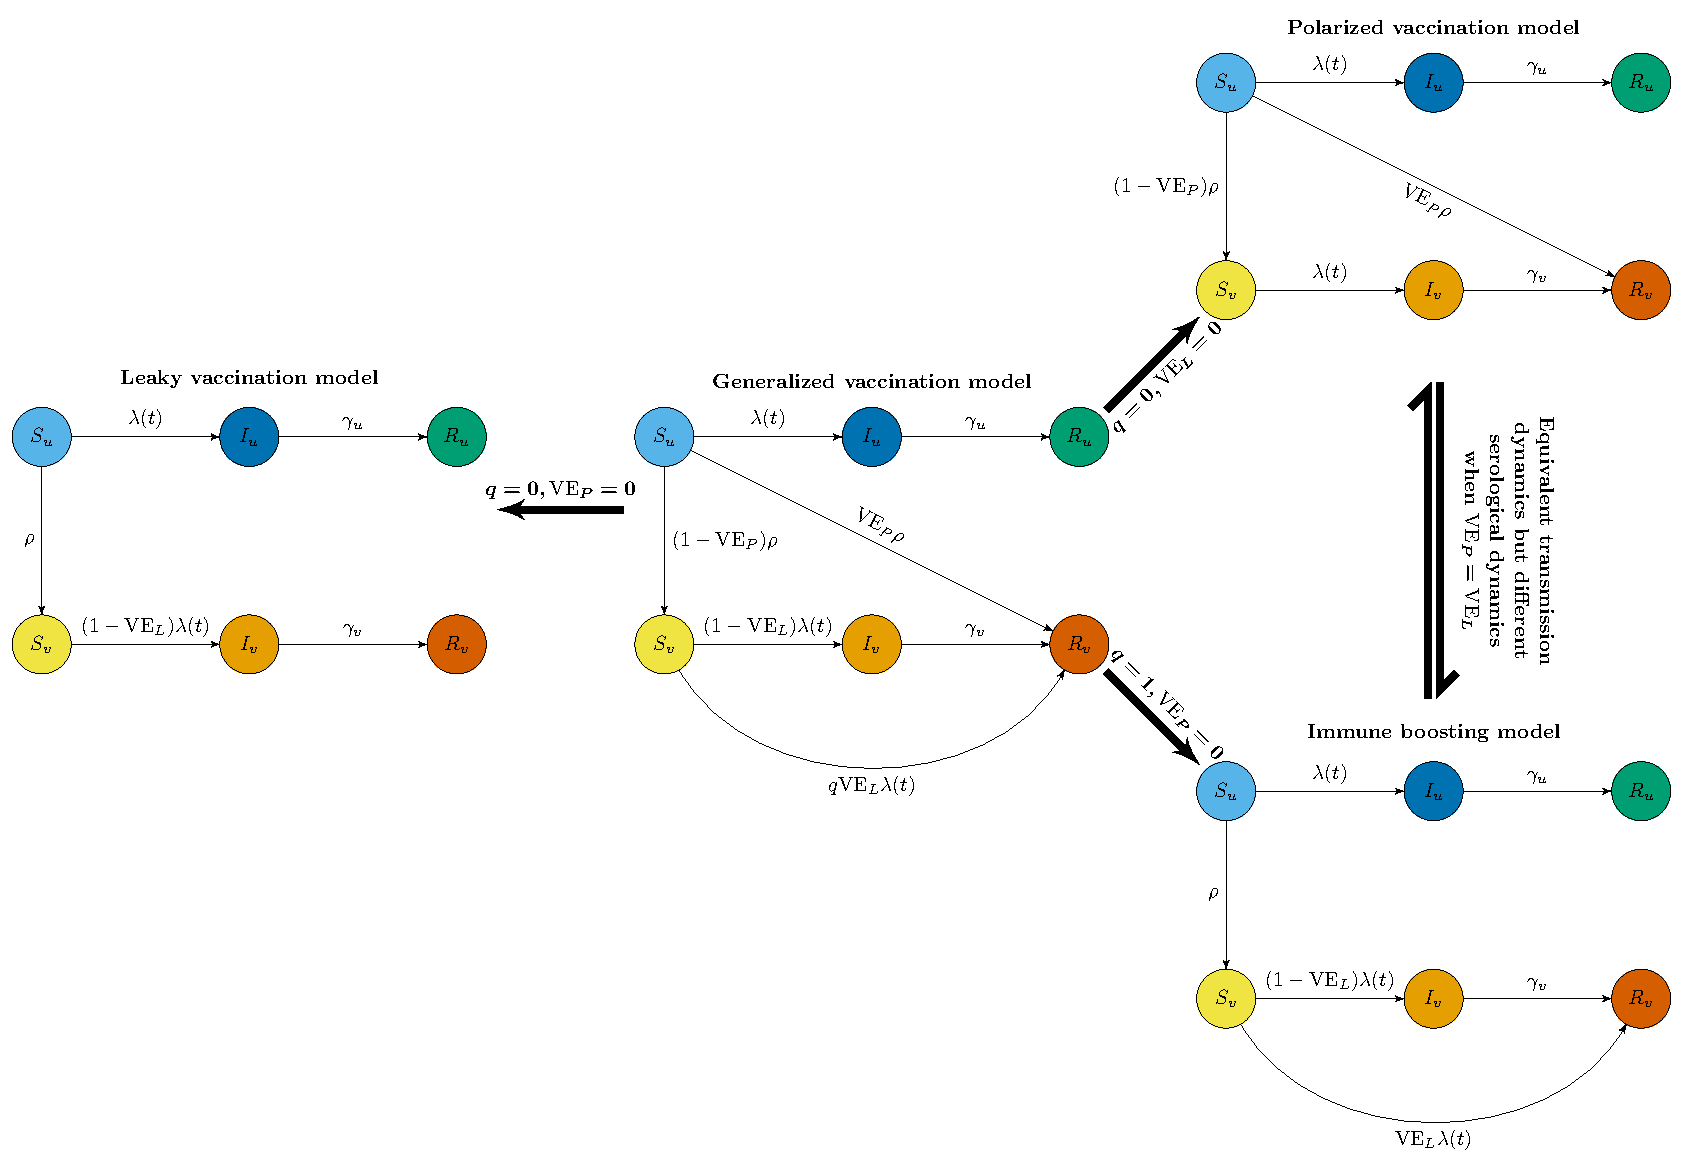
\includegraphics[width=\textwidth]{figure_diagram_comb.pdf}
\caption{
\textbf{A schematic diagram of vaccine models}
\label{fig:diagram}
}
\end{figure}

First, we begin with a standard SIR model with a leaky vaccine, in which all vaccinated individuals experience a reduced force of infection by a factor of $p$:
\begin{align}
\frac{\dd S}{\dd t} &= - \lambda(t) S - \rho S \\
\frac{\dd I_u}{\dd t} &= \lambda(t) S - \gamma_u I_u \\
\frac{\dd R_u}{\dd t} &= \gamma_u I_u \\
\frac{\dd V}{\dd t} &= - p \lambda(t) V + \rho S \\
\frac{\dd I_v}{\dd t} &= p \lambda(t) V - \gamma_v I_v \\
\frac{\dd R_v}{\dd t} &= \gamma_v I_v
\end{align}
where $\lambda$ represents the baseline force of infection experienced by unvaccinated individuals; $\rho$ represents vaccination rate; and $\gamma_u$ and $\gamma_v $ represent the recovery of the unvaccinated and vaccinated individuals, respectively.
This kind of model is also referred to as a history-based model as the susceptibility of an individual depends on the history of infections or vaccination---in this case, all individuals who have the same vaccine history have identical susceptibility.

On the other hand, the polarized vaccination model assumes that a proportion $p$ of vaccinated individuals still remain susceptible, whereas the remaining proportion $1-p$ become fully immune: 
\begin{align}
\frac{\dd S}{\dd t} &= - \lambda(t) S - \rho S \\
\frac{\dd I_u}{\dd t} &= \lambda(t) S - \gamma_u I_u \\
\frac{\dd R_u}{\dd t} &= \gamma_u I_u \\
\frac{\dd V}{\dd t} &= - \lambda(t) V + p \rho S \\
\frac{\dd I_v}{\dd t} &= \lambda(t) V - \gamma_v I_v \\
\frac{\dd R_v}{\dd t} &= \gamma_v I_v + (1-p) \rho S
\end{align}
The polarized immunity model is often used in status-based models for cross immunity---the status-based models keep track of immune statuses of individuals, rather than their infection histories.

While both the leaky vaccination model and the polarized vaccination model have been widely used in literature, their assumptions lead to a key dynamical differences: the leaky vaccination model assumes that all vaccinated individuals can be eventually infected, whereas the polarized vaccination model assumes that proportion $1-p$ of vaccinated individuals will never be infected.
In other words, the polarized vaccination model will always predict a lower final size than the leaky vaccination model.

To better understand these differeces, we consider a immune boosting model.
The leaky vaccination model assumes that vaccinated individuals have an independent probability $p$ of infection for every challenge and will otherwise remain partially susceptible.
Instead, the immune boosting model assumes that unsuccessful challenges elicit immune response, moving individuals from $V$ to $R_v$ compartment at rate $(1-p) \lambda(t)$ and thereby breaking the independence assumption: 
\begin{align}
\frac{\dd S}{\dd t} &= - \lambda(t) S - \rho S \\
\frac{\dd I_u}{\dd t} &= \lambda(t) S - \gamma_u I_u \\
\frac{\dd R_u}{\dd t} &= \gamma_u I_u \\
\frac{\dd V}{\dd t} &= - \lambda(t) V + \rho S \\
\frac{\dd I_v}{\dd t} &= p \lambda(t) V - \gamma_v I_v \\
\frac{\dd R_v}{\dd t} &= (1-p) \lambda(t) V + \gamma_v I_v
\end{align}
In this model, both unvaccinated and vaccinated individuals are subject to identical forces of infections, which represent the per capita rate of challenges, but the outcome of challenges differ.
Since the depletion of vaccinated population $V$ always occurs at a faster rate under the immune boosting model than under the leaky vaccination model, the immune boosting model always predicts a lower final size.
Furthermore, epidemiological dynamics (i.e., trajectories of $I_u$ and $I_v$) predicted by the immune boosting model and the polarized vaccination model are identical: 
both models assume that individuals become vaccinated at rate $\rho$ and move out of the $V$ compartment at rate $\lambda$ and only differ in when individuals get sorted.
Such equivalence allows us to bridge the difference between the leaky and polarized vaccination models.
The equivalence holds regardless of infection characteristics of vaccinated individuals (i.e., the duration of their infection and their transmissibility);
however, it does not hold when immunity wanes as we show later.

Finally, we present a generalized vaccination model that encompasses all three models:
\begin{align}
\frac{\dd S}{\dd t} &= - \lambda(t) S - \rho S \\
\frac{\dd I_u}{\dd t} &= \lambda(t) S - \gamma_u I_u \\
\frac{\dd R_u}{\dd t} &= \gamma_u I_u \\
\frac{\dd V}{\dd t} &= - [q \{1-(p/\theta)\} + (p/\theta)] \lambda(t) V + \theta \rho S \\
\frac{\dd I_v}{\dd t} &= (p/\theta) \lambda(t) V - \gamma_v I_v \\
\frac{\dd R_v}{\dd t} &= (1 - \theta) \rho S + q [1-(p/\theta)] \lambda(t) V + \gamma_v I_v
\end{align}
This model includes two additional parameters: $\theta$ and $q$.
The parameter $\theta$ represents the proportion of individuals that remain partially susceptible after vaccination;
this paramter also scales the force of infection, allowing us to bridge the polarized vaccination and immune boosting models.
For example, when $\theta = 1$, all vaccinated individuals are partially susceptible to breakthrough infections;
the value of paramter $q$, which represents the proportion of unsuccessful challenges that result in immune boosting, then allow us to bridge between the leaky vaccination model ($q=0$) and the immune boosting model ($q = 1$).
When $\theta = p$, a proportion $p$ of vaccinated individuals are completely susceptible to breakthrough infections, yielding a polarized vaccination model.
We note that this generalized model does not account for the possibility that a proportion $p$ of vaccinated individuals remain partially susceptible to breakthrough infections while the remaining proportion $1-p$ of vaccinated individuals are completely protected; 
as we discuss later, a such model would violate the definition of vaccine efficacy against infection \swp{need to reword this and stress this earlier on}.
These four models are summarized in \fref{diagram}.

\section{Model simulations}


As an example, we assume that both unvaccinated and vaccinaed individuals transmit at the same rate for an average of 5 days with $\mathcal R_0 = 2.5$ in a homogeneously mixing population.
For simplicity, we assume that 50\% individuals are vaccinated at the beginning of an epidemic with 60\% efficacy ($p=0.4$) and do not model vaccination during an outbreak ($\rho = 0$).
For the leaky vaccination model and the immune boosting model, we set $V(0) = 0.5$ as our initial condition;
for the polarized vaccination model, we set $V(0) = 0.5 p$ and $R_v(0) = 0.5 (1-p)$ as our initial condition.

\fref{simulation} compares epidemiological (A--C) and serological (D--F) trajectories predicted by three models (leaky vaccination model, polarized vaccination model, and immune boosting model).
As shown earlier, the leaky vaccination model predicts a larger outbreak with a slower decay rate among vaccinated individuals than predicted by both the polarized vaccination and immune boosting models;
the latter two models predict identical epidemic trajectories.
In this case, the leaky vaccination model also predicts a larger outbreak among unvaccinated individuals because a larger outbreak among vaccinated individuals causes unvaccinated individuals to also experience a greater forces of infection over time.

We also find that all three models predict different serological trajectories. (\fref{simulation}D--F).
The leaky vaccination model predicts the largest outbreak and therefore the highest levels of seroprevalence.
The immune boosting model predicts a slightly lower seroprevalence overall;
in addition, a higher proportion of vaccinated individuals have moved from $V$ to $R_v$ compartment through boosting.


\begin{figure}[!th]
\includegraphics[width=\textwidth]{figure_simulation_compare.pdf}
\caption{
\textbf{Simulations of three different vaccination models}
\label{fig:simulation}
}
\end{figure}



\begin{figure}[!th]
\includegraphics[width=\textwidth]{figure_simulation_generalized_vaccinated.pdf}
\caption{
\textbf{Sensitivity of the final size of an outbreak among vaccinated individuals to assumptions about vaccine-derived immunity}
\label{fig:new}
}
\end{figure}


\begin{figure}[!th]
\includegraphics[width=\textwidth]{figure_simulation_effectiveness.pdf}
\caption{
\textbf{Sensitivity of the final size of an outbreak among vaccinated individuals to assumptions about vaccine-derived immunity}
\label{fig:new2}
}
\end{figure}


\end{document}
